\Chapter{Fejlesztés}

\Section{Fejlesztés előkészítése}

Miután kialakult egy konkrét elképzelés a szakdolgozat témájával kapcsolatosan, összegyűjtöttem a legfontosabb szempontokat, hogy mikre kell a legnagyobb figyelmet fordítanom a program implementálása során. Alaposan átolvastam a Monopoly játék eredeti szabályait \cite{coombs1987markup}, és az általam elgondolt online megvalósítás lehetőségeivel összefésültem. Célom ezzel az volt, hogy a játék online verzióban is izgalmas, kiegyensúlyozott élményt nyújtson. Készítettem egy tervet a játék megvalósításának lépéseiről, ami nagyban segített abban, hogy hol lesznek esetleges nehézségek a fejlesztés során.

Ennek a folyamatábrának a megalkotásával próbáltam megtervezni, hogy hogyan fog kinézni maga a játék menete programozási szempontból. Elkészítéséhez a draw.io nevezetű folyamatábra készítő ingyenes internetes programot használtam, mely nagyban megkönnyítette a feladatomat a fejlesztés további szakaszaiban.

A backend illetve a frontend részek megírása párhuzamosan ment, mivel így lehetőség adódott teljes értékű funkciókat kipróbálni már az előtt, hogy a teljes frontend vagy backend elkészült volna. Ebből kifolyólag a tesztelési fázisok is azonnal megtörténtek, így az előforduló hibákat kisebb kód részben kellett keresnem és javítanom. Abban az esetben, ha a programnak több komponensét szerettem volna összekapcsolni előfordult, hogy néhány függvényt vagy osztályt egy az egyben újra kellett gondolnom. Ezeket a lépéseket folyamatosan dokumentáltam, ami segített abban, hogy utólag visszaolvasva is lássam, hogy mit miért kellett javítanom.


\begin{figure}[h!]
\centering
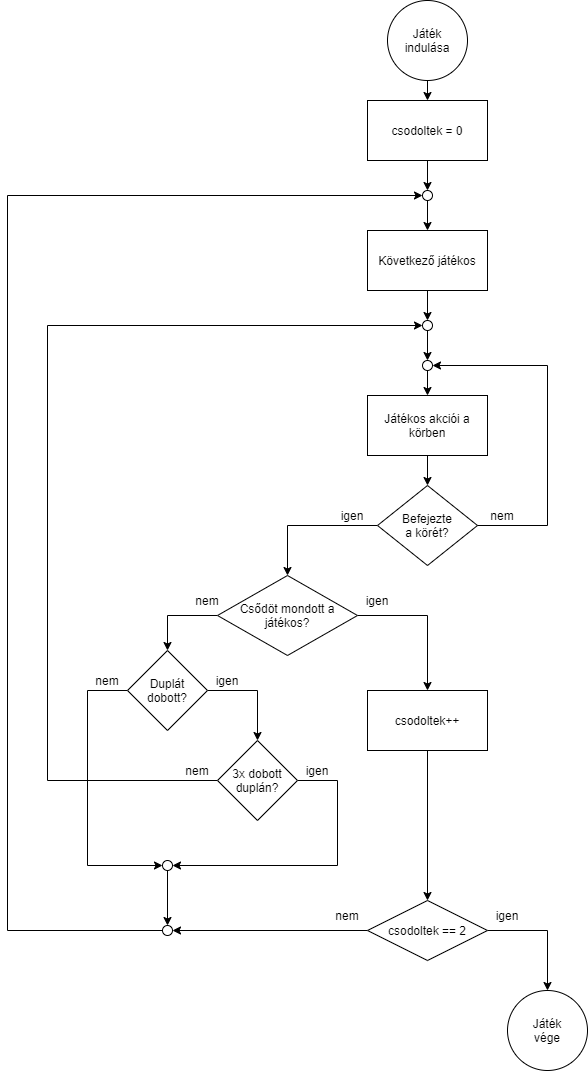
\includegraphics[scale=0.6]{images/folyamata.png}
\caption{A játék folyamatábrája}
\label{fig:ff}
\end{figure}
\newpage
\Section{Fejlesztés menete}

Az első lépések közé tartozott a NodeJS szoftverrendszer telepítése, illetve a VueJS javascript keretrendszer npm-el történő installálása.

	Ezután létrehoztam egy teljesen alap, sablon Vue projektet, ami a későbbiekben magának a frontend résznek az alapját képezi. Ezzel együtt egy server.js fájlt is elkészítettem, mely magát a szervert alkotja egy express keretrendszer segítségével. Miután ezek a lépések megtörténtek, beépítettem a socket.io nevezetű valós idejű kliens-szerver kommunikációt segítő javascript keretrendszert. Erre azért volt szükség, mert a tervezési fázisban már tudtam, hogy szükségem lesz arra, hogy a szerver több klienst is ki tudjon szolgálni egyszerre valós időben.

	Felhasználói szempontból az első feladat egy bejelentkező felület elkészítése volt. Ennek megvalósításához egy Login.vue komponenst hoztam létre és importáltam az App.vue alkalmazásba. A Login.vue-n keresztül kapott adatokat át kellett adni az App.vue-nak, hogy az továbbítani tudja a szerver felé ezeket, hiszen maga a komponens nem áll kapcsolatban közvetlen a szerverrel. Az elsőként bejelentkezett játékos a HOST titulust viseli, ő indítja a játékot, illetve képes parancsok használatára.

	Szükség volt egy Chat megvalósítására ahol a játékosok információkat látnak a játékkal kapcsolatban, illetve kommunikálni is tudnak egymással. Ezt a felületet használtam arra is, hogy jobban megismerkedjek a socket.io lehetőségeivel, és tesztelni tudjam annak működését. Ezen a felületen van lehetősége a HOST-nak parancsok kiadására (pl.: ‘/start’ - A játék indítása).

	A játék kezdete előtt a játékosok egy úgynevezett várakozó szobába kerülnek, ezért a következő teendő ennek az elkészítése volt. Lényegében erre azért volt szükség, hogy összegyűljön a négy játékos a játék kezdetéhez.

	A grafikus felület elkészítése is fontos része volt a folyamatnak. Egy átlátható, könnyen kezelhető alkalmazás létrehozása volt a célom. Törekedtem az egyedi megvalósításokra, a webes megjelenítésekhez Bootstrap keretrendszert, illetve egyéni css-t alkalmaztam. A képi elemek megvalósításához az Adobe Photoshop 2020 nevezetű programot használtam, már itt fontosnak tartottam azt, hogy mindenből meglegyen a .psd fájl is, ha esetlegesen szerkesztenem kellene.

	A szerveren belül megvalósítottam, hogy tárolja a bejelentkezett játékosokat, és folyamatosan frissítse azok állapotát minden kliens felületén. A program ezen állapotában még csak egy players nevű tömb tárolta a játékosok paramétereit, és a játék állását pedig változók a server.js-n belül.

	Elkészítettem a Table.vue komponenst, ami megjeleníti a játék aktuális állását, a táblát és a rajta elhelyezkedő bábúk helyzetét. Emellett ebben a komponensben helyeztem el a játékos által használható gombokat (pl.: “Dobás” - Dobás a kockával). Ebben a fejlesztési szakaszban került sor arra is, hogy paraméterezzem a bábúk helyzetét az aktuális mezőre lépéskor, ez viszonylag aprólékos feladat volt. A szerverben megvalósításra került a következő aktív játékos beállítása, illetve frissítése a kliensek számára is. A szabályzathoz igazítva a dupla illetve tripla dobások lehetőségét is figyelembe véve. Itt több tesztelésre is sor került, ez a fázis tekinthető a játék első prototipusának. Ekkorra éreztem azt, hogy kellően megismertem a használt keretrendszerek lehetőségeit.

	A program elérkezett abba a fázisba, hogy objektum orientált legyen. Létrehoztam külön osztályokat a classes mappába. Ezek voltak a Game, Player, PlayerManager, Property, Table nevezetű osztályok. A szerveren belül illetve az App.vue-ban is ezeknek megfelelően lettek átgondolva az eddig megvalósított funkciók, és sokkal átláthatóbb lett a kódolás.

	Egy nagyobb fejlesztés következett, a bizniszek kidolgozása. Minden ezzel kapcsolatos dolog megvalósításra került (vásárlás,fizetés,eladás). Ennek mintájaként a telkek, illetve szolgáltatók is hasonlóképpen készültek el, hiszen a logikai felépítésük nem tért el sokban.

	A kereskedés funkció volt az utolsó dolog ami nagyobb kihívást jelentett számomra, hiszen itt két játékos közötti kommunikációt kellett megvalósítani a szerveren keresztül. Ennek a megvalósítása viszonylag időigényes volt, de mire idáig eljutottam a fejlesztésben már kellő tapasztalatra tettem szert az alkalmazást illetően.

Innen már csak apróságok választottak el az 1.0-s verziótól, ezek pedig inkább a kreatív dolgok voltak. Kitaláltam a mezőneveket, illetve hogy mik szerepeljenek a szerencsekártyákon (illetve ezeket leprogramozni).

Utolsó simításként a játék vége, a csőd megalkotása maradt hátra, ami egy nagyon egyszerű folyamatként sikerült, és mivel elsőre sikerült úgy megírni ahogy elterveztem, jöhetett is magánk a játéknak a tesztelése, egyelőre még csak botok nélkül.

A tesztelés úgy zajlott, hogy négyen játszottunk külön eszközökről, ugyanarról a hálózatról. Körülbelül maga a tesztelés 4-5 órát vett igénybe, nagyjából 10-14 játékot játszottunk, viszont valamelyik csak pár percig tartott a talált problémák miatt. Azokat a hibákat, amik befolyásolták a játék menetét rögtön javítottam.

Ilyen volt például, hogy az alkalmazás rosszul kezelte a kör átadását tripla dobás esetén. Viszont ami csak úgymond formailag tett hozzá a játékhoz, azokat kigyűjtöttük egy lapra, hogy a tesztelés után sorban tudjam javítani a felírt dolgokat, emellett az is felkerült a papírra, hogy hol és mikor jelentkeztek az adott hibák. Amikor a talált hibák kijavításra kerültek, elkezdődött a botok megírása.

Kezdetben egy olyan botra volt szükségem, ami képes alap funkciók végrehajtására. Ezalatt a dobást, kör átadását, illetve a börtönből való szabadulást, csődöt értem. Külön osztályt kapott BotEasy néven, és tudtam, hogy a továbbiakban ezt fogom továbbfejleszteni. Három különböző nehézségű bot megvalósítását terveztem, így el kellett döntenem, milyen funkciókban fognak főként eltérni egymástól.

Soron következő megvalósítású botom a BotMedium osztályt kapta. Már képes volt a táblán lévő összes megvásárolható biznisz/szolgáltatás/telek megvételére, és válogatás nélkül élt is a lehetőséggel. Lehetőséget adtam neki, hogy fejleszteni illetve bontani tudja a telkeket, esetenként eladni azokat, hogyha csőd közeli helyzetbe kerül.

Végezetül, a legerősebb bot a BotHard osztályt tudhatja magáénak. Nagyban hasonlít a BotMedium osztályra, viszont ők már paraméterezve vannak. Kialakításuk során gondolnom kellett arra, hogy a leendő szimulációkban ők foglalnak majd helyet.

\newpage
\Section{Filestruktúra felépítése}

Ebben az alfejezetben kerül bemutatásra az alkalmazás mappaszerkezete egy listával ábrázolva.

\renewcommand{\labelitemi}{$\blacksquare$}
 \renewcommand\labelitemii{$\square$}
 \begin{itemize}
   \item  classes - Alkalmazáshoz írt osztályok.
   \item simulations - Lefuttatott szimulációk.
\item client - Frontend megvalósítás VueJS keretrendszerrel.

   \begin{itemize}
     \item  public - index.html és társai
     \item src - Vue app gyökérmappája
     \begin{itemize}
       \item  assets - Megjelenítendő dolgok
	\item components - Vue app komponensei

     \end{itemize}
   \end{itemize}
 \end{itemize}
